\setlength{\footskip}{8mm}
%\mainmatter
\chapter{Introduction}

\section{Background}


Cameras are everywhere, in front of stores, businesses and on our streets. They are used for several purposes:\begin{itemize}
\item After a crime has been commited, the video can be used as clues or proof. The goal is to get more information on the person or on the event that has occurred.
\item In the few minutes after a crime, to intercept the person who committed it. Some police are always scanning surveillance videos, monitoring subways, streets, and so on to be able to catch the perpetrator in the corridor or before he or she could escape.
\item Before a crime, typically, to dissuade potential thieves from stealing anything. Sometimes, even cameras that are not working, not recording, or are fakes can be effetive deterrents.
\end{itemize}

In the context of global terrorism, the problem of recognizing a previously identified terrorist, hoping to follow him or her through video cameras through several feeds sadly appears to be a key issue. More generally, following the path of any criminal using surveillance videos sounds like a main concern.\\

In this work we can assume that police face several difficulties:\begin{itemize}
\item The number of cameras they may have access to, depending on the locality's policy. This number may be very high, and is growing everywhere very quickly.
\item The low quality of the video. It is sometimes very hard to recognize a person in a video with low resolution.
\item The crowd. It takes a second to recognize a previously identified thief on a video when he or she is alone. What if there are 30 other people on the video, in a crowded street for example?
\end{itemize}

Recognizing previously identified criminals in video surveillance feeds adds to the above-mentioned difficulties, requiring a great deal of human resources. These issues lead to a simple conclusion.  It is expensive work in terms of time, money, and human resources, but it is nevertheless extremely important to uphold the national security of any country.\\

Automating the face recognition process in surveillance video seems to be an interesting answer to address some of these problems.\\


\section{Problem Statement}

 Face identification is a key machine learning issue at present. The best results obtained this far use a \enquote{deep} neural network (any artificial neural network with more than one hidden layer). In 2014, DeepFace reached an accuracy of 97.35\% on \enquote{the Labeled Faces in the Wild (LFW)} dataset for face verification (Taigman, Yang, Ranzato, Wolf, 2014). In 2015, FaceNet reached a 99.63\% accuracy on the \enquote{LFW} dataset for identification (Schroff, Kalenichenko, Philbin, 2015).\\


In surveillance video, face recognition faces difficult issues such as blurriness, low resolution, and unexpected poses of faces. Though the problem of face recognition in surveillance video has already been studied, deep learning techniques may improve performance in this scenario.\\

The goal of this research was to build a deep neural network for face recognition on surveillance videos. This model had to be based on the latest algorithms and best practices deep learning offers.

\section{Objectives}

The objectives of this research were to develop and evaluate methods for a database already provided for the study. This database contained recorded videos from the surveillance camera network at the MBK shopping mall in Bangkok. Figure 1.1 shows a frame of one of these videos. Three of our researchers appeared over several seconds in some of the videos. They were walking like anyone else in the mall.\\

\begin{figure}[t]
  \centering
  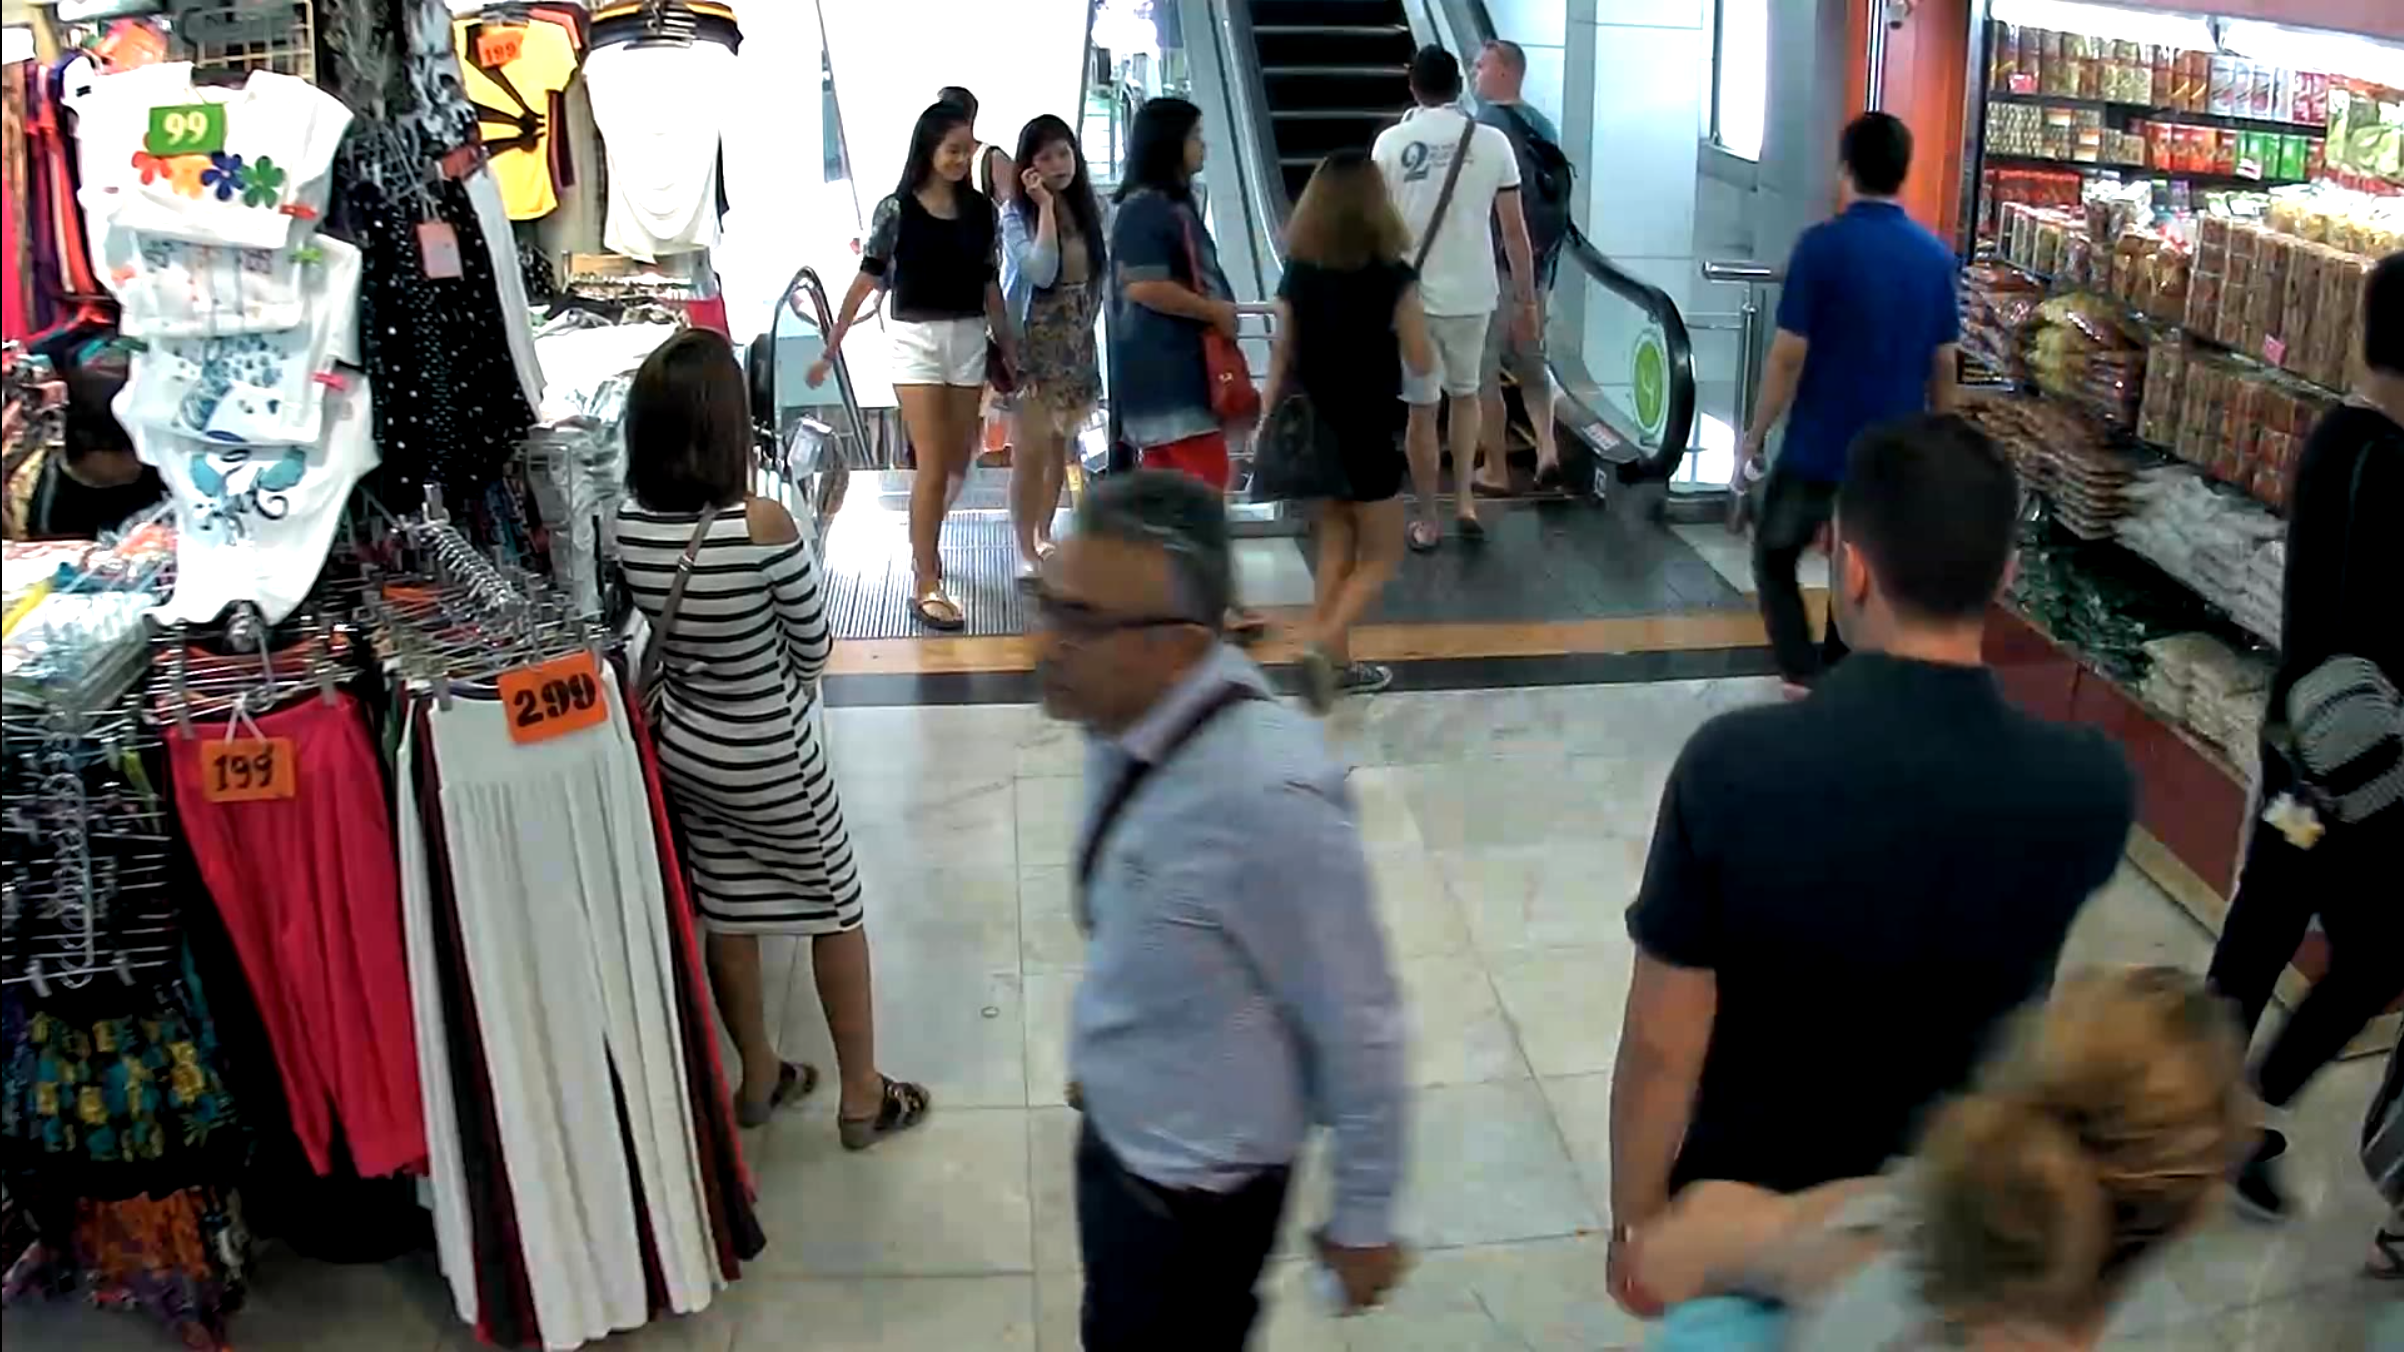
\includegraphics[scale=0.3]{figures/database.png}  
  \caption[A frame from a video in the MBK dataset.]{A frame from a video in the MBK dataset.}
  \label{fig:example}
\end{figure}

Choosing this database served one goal: to be placed in the theoretical situation of policemen looking for one or several criminals in the streets or in the corridors of public places, using a few sample pictures of them to try to track and find out where they have gone.\\

Our researchers are playing the role of the criminals we are looking for.
The main objective was to use deep learning techniques to build an automated solution for the task of finding people we have a few photos of over a larger collection of video streams.\\

More precisely, considering this database, there were three main objectives in this research study:
\begin{itemize}
\item Create a database of images containing faces extracted from the surveillance videos.
\item Build a deep neural network for face recognition. The general idea is that the network should be provided with a few photos of our researchers from a training set, and try to find these individuals in a testing set.
\item Testing the resulting model. Compare the model's accuracy with other experiments using different techniques.
\end{itemize}

\section{Limitations and Scope}

There were two main limitations to this research:
\begin{itemize}
\item Time. This project was three months long. There are many deep learning techniques existing, but due to the time limit, not all could be explored.
\item Material limitations. The laboratory has provided a single NVIDIA GeForce 780 GTX GPU card for the computation. This places some limitations on the mini-batch size for stochastic gradient descent. Preliminary results showed that the size will be limited to 20 samples, while the usual size is 128.
\end{itemize}

Deep learning gives astonishing results in the task of face recognition. That is why despite those limitations, we were able to get an interesting model for the context of surveillance videos.

\section{Research Outline}

I organize the rest of this dissertation as follows.

In Chapter \ref{ch:literature-review}, I provide a review of the relevant literature.

In Chapter \ref{ch:methodology}, I propose my methodology.

In Chapter \ref{ch:results}, I present the results of the study.

Finally, in Chapter \ref{ch:conclusion}, I conclude my thesis.

\FloatBarrier